\documentclass[10pt]{article} 
\usepackage[margin=0.73in]{geometry}
\usepackage{amsmath}
\usepackage{hyperref} 
\usepackage{listings}
\usepackage{xcolor}
\usepackage{multicol}
\usepackage{graphicx}
\usepackage{float}

\RequirePackage{color}
\RequirePackage{listings}

\lstdefinelanguage{Rust}{%
  sensitive%
, morecomment=[l]{//}%
, morecomment=[s]{/*}{*/}%
, moredelim=[s][{\itshape\color[rgb]{0,0,0.75}}]{\#[}{]}%
, morestring=[b]{"}%
, alsodigit={}%
, alsoother={}%
, alsoletter={!}%
%
%
% [1] reserve keywords
% [2] traits
% [3] primitive types
% [4] type and value constructors
% [5] identifier
%
, morekeywords={break, continue, else, for, if, in, loop, match, return, while}  % control flow keywords
, morekeywords={as, const, let, move, mut, ref, static}  % in the context of variables
, morekeywords={dyn, enum, fn, impl, Self, self, struct, trait, type, union, use, where}  % in the context of declarations
, morekeywords={crate, extern, mod, pub, super}  % in the context of modularisation
, morekeywords={unsafe}  % markers
, morekeywords={abstract, alignof, become, box, do, final, macro, offsetof, override, priv, proc, pure, sizeof, typeof, unsized, virtual, yield}  % reserved identifiers
%
% grep 'pub trait [A-Za-z][A-Za-z0-9]*' -r . | sed 's/^.*pub trait \([A-Za-z][A-Za-z0-9]*\).*/\1/g' | sort -u | tr '\n' ',' | sed 's/^\(.*\),$/{\1}\n/g' | sed 's/,/, /g'
, morekeywords=[2]{Add, AddAssign, Any, AsciiExt, AsInner, AsInnerMut, AsMut, AsRawFd, AsRawHandle, AsRawSocket, AsRef, Binary, BitAnd, BitAndAssign, Bitor, BitOr, BitOrAssign, BitXor, BitXorAssign, Borrow, BorrowMut, Boxed, BoxPlace, BufRead, BuildHasher, CastInto, CharExt, Clone, CoerceUnsized, CommandExt, Copy, Debug, DecodableFloat, Default, Deref, DerefMut, DirBuilderExt, DirEntryExt, Display, Div, DivAssign, DoubleEndedIterator, DoubleEndedSearcher, Drop, EnvKey, Eq, Error, ExactSizeIterator, ExitStatusExt, Extend, FileExt, FileTypeExt, Float, Fn, FnBox, FnMut, FnOnce, Freeze, From, FromInner, FromIterator, FromRawFd, FromRawHandle, FromRawSocket, FromStr, FullOps, FusedIterator, Generator, Hash, Hasher, Index, IndexMut, InPlace, Int, Into, IntoCow, IntoInner, IntoIterator, IntoRawFd, IntoRawHandle, IntoRawSocket, IsMinusOne, IsZero, Iterator, JoinHandleExt, LargeInt, LowerExp, LowerHex, MetadataExt, Mul, MulAssign, Neg, Not, Octal, OpenOptionsExt, Ord, OsStrExt, OsStringExt, Packet, PartialEq, PartialOrd, Pattern, PermissionsExt, Place, Placer, Pointer, Product, Put, RangeArgument, RawFloat, Read, Rem, RemAssign, Seek, Shl, ShlAssign, Shr, ShrAssign, Sized, SliceConcatExt, SliceExt, SliceIndex, Stats, Step, StrExt, Sub, SubAssign, Sum, Sync, TDynBenchFn, Terminal, Termination, ToOwned, ToSocketAddrs, ToString, Try, TryFrom, TryInto, UnicodeStr, Unsize, UpperExp, UpperHex, WideInt, Write}
, morekeywords=[2]{Send}  % additional traits
%
, morekeywords=[3]{bool, char, f32, f64, i8, i16, i32, i64, isize, str, u8, u16, u32, u64, unit, usize, i128, u128}  % primitive types
%
, morekeywords=[4]{Err, false, None, Ok, Some, true}  % prelude value constructors
% grep 'pub \(type\|struct\|enum\) [A-Za-z][A-Za-z0-9]*' -r . | sed 's/^.*pub \(type\|struct\|enum\) \([A-Za-z][A-Za-z0-9]*\).*/\2/g' | sort -u | tr '\n' ',' | sed 's/^\(.*\),$/{\1}\n/g' | sed 's/,/, /g'    
, morekeywords=[3]{AccessError, Adddf3, AddI128, AddoI128, AddoU128, ADDRESS, ADDRESS64, addrinfo, ADDRINFOA, AddrParseError, Addsf3, AddU128, advice, aiocb, Alignment, AllocErr, AnonPipe, Answer, Arc, Args, ArgsInnerDebug, ArgsOs, Argument, Arguments, ArgumentV1, Ashldi3, Ashlti3, Ashrdi3, Ashrti3, AssertParamIsClone, AssertParamIsCopy, AssertParamIsEq, AssertUnwindSafe, AtomicBool, AtomicPtr, Attr, auxtype, auxv, BackPlace, BacktraceContext, Barrier, BarrierWaitResult, Bencher, BenchMode, BenchSamples, BinaryHeap, BinaryHeapPlace, blkcnt, blkcnt64, blksize, BOOL, boolean, BOOLEAN, BoolTrie, BorrowError, BorrowMutError, Bound, Box, bpf, BTreeMap, BTreeSet, Bucket, BucketState, Buf, BufReader, BufWriter, Builder, BuildHasherDefault, BY, BYTE, Bytes, CannotReallocInPlace, cc, Cell, Chain, CHAR, CharIndices, CharPredicateSearcher, Chars, CharSearcher, CharsError, CharSliceSearcher, CharTryFromError, Child, ChildPipes, ChildStderr, ChildStdin, ChildStdio, ChildStdout, Chunks, ChunksMut, ciovec, clock, clockid, Cloned, cmsgcred, cmsghdr, CodePoint, Color, ColorConfig, Command, CommandEnv, Component, Components, CONDITION, condvar, Condvar, CONSOLE, CONTEXT, Count, Cow, cpu, CRITICAL, CStr, CString, CStringArray, Cursor, Cycle, CycleIter, daddr, DebugList, DebugMap, DebugSet, DebugStruct, DebugTuple, Decimal, Decoded, DecodeUtf16, DecodeUtf16Error, DecodeUtf8, DefaultEnvKey, DefaultHasher, dev, device, Difference, Digit32, DIR, DirBuilder, dircookie, dirent, dirent64, DirEntry, Discriminant, DISPATCHER, Display, Divdf3, Divdi3, Divmoddi4, Divmodsi4, Divsf3, Divsi3, Divti3, dl, Dl, Dlmalloc, Dns, DnsAnswer, DnsQuery, dqblk, Drain, DrainFilter, Dtor, Duration, DwarfReader, DWORD, DWORDLONG, DynamicLibrary, Edge, EHAction, EHContext, Elf32, Elf64, Empty, EmptyBucket, EncodeUtf16, EncodeWide, Entry, EntryPlace, Enumerate, Env, epoll, errno, Error, ErrorKind, EscapeDebug, EscapeDefault, EscapeUnicode, event, Event, eventrwflags, eventtype, ExactChunks, ExactChunksMut, EXCEPTION, Excess, ExchangeHeapSingleton, exit, exitcode, ExitStatus, Failure, fd, fdflags, fdsflags, fdstat, ff, fflags, File, FILE, FileAttr, filedelta, FileDesc, FilePermissions, filesize, filestat, FILETIME, filetype, FileType, Filter, FilterMap, Fixdfdi, Fixdfsi, Fixdfti, Fixsfdi, Fixsfsi, Fixsfti, Fixunsdfdi, Fixunsdfsi, Fixunsdfti, Fixunssfdi, Fixunssfsi, Fixunssfti, Flag, FlatMap, Floatdidf, FLOATING, Floatsidf, Floatsisf, Floattidf, Floattisf, Floatundidf, Floatunsidf, Floatunsisf, Floatuntidf, Floatuntisf, flock, ForceResult, FormatSpec, Formatted, Formatter, Fp, FpCategory, fpos, fpos64, fpreg, fpregset, FPUControlWord, Frame, FromBytesWithNulError, FromUtf16Error, FromUtf8Error, FrontPlace, fsblkcnt, fsfilcnt, fsflags, fsid, fstore, fsword, FullBucket, FullBucketMut, FullDecoded, Fuse, GapThenFull, GeneratorState, gid, glob, glob64, GlobalDlmalloc, greg, group, GROUP, Guard, GUID, Handle, HANDLE, Handler, HashMap, HashSet, Heap, HINSTANCE, HMODULE, hostent, HRESULT, id, idtype, if, ifaddrs, IMAGEHLP, Immut, in, in6, Incoming, Infallible, Initializer, ino, ino64, inode, input, InsertResult, Inspect, Instant, int16, int32, int64, int8, integer, IntermediateBox, Internal, Intersection, intmax, IntoInnerError, IntoIter, IntoStringError, intptr, InvalidSequence, iovec, ip, IpAddr, ipc, Ipv4Addr, ipv6, Ipv6Addr, Ipv6MulticastScope, Iter, IterMut, itimerspec, itimerval, jail, JoinHandle, JoinPathsError, KDHELP64, kevent, kevent64, key, Key, Keys, KV, l4, LARGE, lastlog, launchpad, Layout, Lazy, lconv, Leaf, LeafOrInternal, Lines, LinesAny, LineWriter, linger, linkcount, LinkedList, load, locale, LocalKey, LocalKeyState, Location, lock, LockResult, loff, LONG, lookup, lookupflags, LookupHost, LPBOOL, LPBY, LPBYTE, LPCSTR, LPCVOID, LPCWSTR, LPDWORD, LPFILETIME, LPHANDLE, LPOVERLAPPED, LPPROCESS, LPPROGRESS, LPSECURITY, LPSTARTUPINFO, LPSTR, LPVOID, LPWCH, LPWIN32, LPWSADATA, LPWSAPROTOCOL, LPWSTR, Lshrdi3, Lshrti3, lwpid, M128A, mach, major, Map, mcontext, Metadata, Metric, MetricMap, mflags, minor, mmsghdr, Moddi3, mode, Modsi3, Modti3, MonitorMsg, MOUNT, mprot, mq, mqd, msflags, msghdr, msginfo, msglen, msgqnum, msqid, Muldf3, Mulodi4, Mulosi4, Muloti4, Mulsf3, Multi3, Mut, Mutex, MutexGuard, MyCollection, n16, NamePadding, NativeLibBoilerplate, nfds, nl, nlink, NodeRef, NoneError, NonNull, NonZero, nthreads, NulError, OccupiedEntry, off, off64, oflags, Once, OnceState, OpenOptions, Option, Options, OptRes, Ordering, OsStr, OsString, Output, OVERLAPPED, Owned, Packet, PanicInfo, Param, ParseBoolError, ParseCharError, ParseError, ParseFloatError, ParseIntError, ParseResult, Part, passwd, Path, PathBuf, PCONDITION, PCONSOLE, Peekable, PeekMut, Permissions, PhantomData, pid, Pipes, PlaceBack, PlaceFront, PLARGE, PoisonError, pollfd, PopResult, port, Position, Powidf2, Powisf2, Prefix, PrefixComponent, PrintFormat, proc, Process, PROCESS, processentry, protoent, PSRWLOCK, pthread, ptr, ptrdiff, PVECTORED, Queue, radvisory, RandomState, Range, RangeFrom, RangeFull, RangeInclusive, RangeMut, RangeTo, RangeToInclusive, RawBucket, RawFd, RawHandle, RawPthread, RawSocket, RawTable, RawVec, Rc, ReadDir, Receiver, recv, RecvError, RecvTimeoutError, ReentrantMutex, ReentrantMutexGuard, Ref, RefCell, RefMut, REPARSE, Repeat, Result, Rev, Reverse, riflags, rights, rlim, rlim64, rlimit, rlimit64, roflags, Root, RSplit, RSplitMut, RSplitN, RSplitNMut, RUNTIME, rusage, RwLock, RWLock, RwLockReadGuard, RwLockWriteGuard, sa, SafeHash, Scan, sched, scope, sdflags, SearchResult, SearchStep, SECURITY, SeekFrom, segment, Select, SelectionResult, sem, sembuf, send, Sender, SendError, servent, sf, Shared, shmatt, shmid, ShortReader, ShouldPanic, Shutdown, siflags, sigaction, SigAction, sigevent, sighandler, siginfo, Sign, signal, signalfd, SignalToken, sigset, sigval, Sink, SipHasher, SipHasher13, SipHasher24, size, SIZE, Skip, SkipWhile, Slice, SmallBoolTrie, sockaddr, SOCKADDR, sockcred, Socket, SOCKET, SocketAddr, SocketAddrV4, SocketAddrV6, socklen, speed, Splice, Split, SplitMut, SplitN, SplitNMut, SplitPaths, SplitWhitespace, spwd, SRWLOCK, ssize, stack, STACKFRAME64, StartResult, STARTUPINFO, stat, Stat, stat64, statfs, statfs64, StaticKey, statvfs, StatVfs, statvfs64, Stderr, StderrLock, StderrTerminal, Stdin, StdinLock, Stdio, StdioPipes, Stdout, StdoutLock, StdoutTerminal, StepBy, String, StripPrefixError, StrSearcher, subclockflags, Subdf3, SubI128, SuboI128, SuboU128, subrwflags, subscription, Subsf3, SubU128, Summary, suseconds, SYMBOL, SYMBOLIC, SymmetricDifference, SyncSender, sysinfo, System, SystemTime, SystemTimeError, Take, TakeWhile, tcb, tcflag, TcpListener, TcpStream, TempDir, TermInfo, TerminfoTerminal, termios, termios2, TestDesc, TestDescAndFn, TestEvent, TestFn, TestName, TestOpts, TestResult, Thread, threadattr, threadentry, ThreadId, tid, time, time64, timespec, TimeSpec, timestamp, timeval, timeval32, timezone, tm, tms, ToLowercase, ToUppercase, TraitObject, TryFromIntError, TryFromSliceError, TryIter, TryLockError, TryLockResult, TryRecvError, TrySendError, TypeId, U64x2, ucontext, ucred, Udivdi3, Udivmoddi4, Udivmodsi4, Udivmodti4, Udivsi3, Udivti3, UdpSocket, uid, UINT, uint16, uint32, uint64, uint8, uintmax, uintptr, ulflags, ULONG, ULONGLONG, Umoddi3, Umodsi3, Umodti3, UnicodeVersion, Union, Unique, UnixDatagram, UnixListener, UnixStream, Unpacked, UnsafeCell, UNWIND, UpgradeResult, useconds, user, userdata, USHORT, Utf16Encoder, Utf8Error, Utf8Lossy, Utf8LossyChunk, Utf8LossyChunksIter, utimbuf, utmp, utmpx, utsname, uuid, VacantEntry, Values, ValuesMut, VarError, Variables, Vars, VarsOs, Vec, VecDeque, vm, Void, WaitTimeoutResult, WaitToken, wchar, WCHAR, Weak, whence, WIN32, WinConsole, Windows, WindowsEnvKey, winsize, WORD, Wrapping, wrlen, WSADATA, WSAPROTOCOL, WSAPROTOCOLCHAIN, Wtf8, Wtf8Buf, Wtf8CodePoints, xsw, xucred, Zip, zx}
%
, morekeywords=[5]{assert!, assert_eq!, assert_ne!, cfg!, column!, compile_error!, concat!, concat_idents!, debug_assert!, debug_assert_eq!, debug_assert_ne!, env!, eprint!, eprintln!, file!, format!, format_args!, include!, include_bytes!, include_str!, line!, module_path!, option_env!, panic!, print!, println!, select!, stringify!, thread_local!, try!, unimplemented!, unreachable!, vec!, write!, writeln!}  % prelude macros
}%

\lstdefinestyle{colouredRust}%
{ basicstyle=\fontsize{9}{9}\ttfamily\selectfont,%
, identifierstyle=%
, commentstyle=\color[gray]{0.4}%
, stringstyle=\color[rgb]{0, 0, 0.5}%
, keywordstyle=\bfseries% reserved keywords
, keywordstyle=[2]\color[rgb]{0.75, 0, 0}% traits
, keywordstyle=[3]\color[rgb]{0, 0.5, 0}% primitive types
, keywordstyle=[4]\color[rgb]{0, 0.5, 0}% type and value constructors
, keywordstyle=[5]\color[rgb]{0, 0, 0.75}% macros
, columns=spaceflexible%
, keepspaces=true%
, showspaces=false%
, showtabs=false%
, showstringspaces=true%
}%

\lstdefinestyle{boxed}{
  style=colouredRust%
, numbers=left%
, firstnumber=auto%
, numberblanklines=true%
, frame=trbL%
, numberstyle=\tiny%
, frame=leftline%
, numbersep=7pt%
, framesep=5pt%
, framerule=10pt%
, xleftmargin=15pt%
, backgroundcolor=\color[gray]{0.97}%
, rulecolor=\color[gray]{0.90}%
}

\title{GxHash: A High-Throughput, Non-Cryptographic Hashing Algorithm Leveraging Modern CPU Capabilities}
\author{Olivier Giniaux}
\date{}

\begin{document}

\maketitle

\begin{abstract}

In the rapidly evolving landscape of data processing and cybersecurity, hashing algorithms play a pivotal role in ensuring data integrity and security.
Traditional hashing methods, while effective, often fail to fully utilize the computational capabilities of modern processors.
This paper introduces the GxHash hashing algorithm, a novel approach that harnesses the power of high Instruction-Level Parallelism (ILP) and Single Instruction, Multiple Data (SIMD) capabilities of contemporary CPUs to achieve high-throughput non-cryptographic hashing. Through a comprehensive analysis, including benchmarks and comparisons with existing methods, we demonstrate that GxHash significantly outperforms conventional algorithms in terms of speed and computational efficiency without compromising on security. The paper also explores the implications, limitations, and avenues for future research in this burgeoning field.

\end{abstract}

\begin{multicols}{2}
\tableofcontents
\end{multicols}

\clearpage
\section{Introduction}

\subsection{Motivations}

As a software engineer at Equativ, a company specializing in high-performance AdServing backends that handle billions of auctions daily,
I face unique challenges in maximizing throughput while minimizing latency. In this high-stakes environment, every millisecond counts, and the performance of underlying data structures becomes critically important. As we heavily rely on in-memory caches and other hash-based data structures, making the efficiency of hashing algorithms a non-trivial concern in our system's overall performance.\\\\
While diving into the theory of hashing out of both necessity and intellectual curiosity, I discovered that existing hashing algorithms, including those built on well-known constructions like Merkle–Damgård, are not optimized to exploit the full capabilities of modern general-purpose CPUs.
These CPUs offer advanced features such as Single Instruction, Multiple Data (SIMD) and Instruction-Level Parallelism (ILP), which remain largely untapped by current hashing methods.\\\\
The challenge of creating a faster, more efficient hashing algorithm became not just a professional necessity but also a personal quest.
It was both challenging and exhilarating to delve into hashing theory and experiment with new approaches. The result is what I believe to be the fastest non-cryptographic hashing algorithm developed to date.\\\\
The primary motivation behind this research is to bridge the existing performance gap by designing a hashing algorithm that fully leverages SIMD and ILP capabilities. The aim is to achieve an order-of-magnitude improvement in hashing speed, thereby revolutionizing the efficiency of various applications, from databases to real-time analytics and beyond.\\\\
In summary, this work is driven by both the practical needs of my professional environment and a personal passion for pushing the boundaries of what is technically possible in the realm of hashing algorithms.

\subsection{Scope Limitation}

\subsubsection{Multithreading}

This paper primarily investigates methods for enhancing the throughput of non-cryptographic hashing algorithms, which are commonly used in a variety of time-sensitive applications, including but not limited to hashmap lookups.
In such contexts, hash computation is often expected to be extremely fast, typically requiring execution times ranging from nanoseconds to microseconds. Given these consideration, the paper intentionally excludes Thread-Level Parallelism
(TLP) as a viable strategy for performance optimization.\\\\
Firstly, it's worth mentioning that TLP is orthogonal to the methods being explored in this paper.
TLP focuses on optimizing coarser-grained operations by distributing tasks across multiple threads, which doesn't directly align with the fine-grained performance improvements we aim to achieve.\\\\
Secondly, introducing TLP would necessitate the incorporation of task scheduling, synchronization, and context switching.
These overheads, while perhaps manageable in applications that can afford greater latencies, become less justifiable when aiming for high-throughput, low-latency operations that are typical in non-cryptographic hashing scenarios.\\\\
In summary, while TLP might be a suitable performance optimization strategy in other computational contexts, we chose to leave it aside in this paper.

\subsubsection{Portability}

Ensuring portability (algorithm generating the same hashes consistently accross different platforms for a given input) is a constrain that may hinder some potential optimization. Our goal being performance first, and our scope of application mainly focused on in-process usages such as hashtables, portability can be left out for these researches. Yet, it remains crutial for the algorithm to work under both x86 and ARM 64-bit platforms that represent most of today's general purpose computing systems.

\clearpage
\section{Related Work}

The field of hashing algorithms has been a subject of extensive research and development, tracing its roots back to foundational architectures like the \textbf{Merkle–Damgård} Construction\cite{merkle}\cite{damgard}, introduced in 1989. Over the years, this area has seen a plethora of innovations, each attempting to address various aspects of hashing—be it collision resistance, distribution uniformity, or computational efficiency. While cryptographic hashing has often been the focal point of research, non-cryptographic hashing algorithms have also garnered attention for their utility in data structures like hashmaps and caches.

In this section, we will explore some of the seminal works and recent advancements in the realm of hashing algorithms to contextualize our research.

\subsection{The Merkle--Damgård Construction}

The Merkle–Damgård construction serves as the foundational architecture for many existing hash functions.
It operates by breaking down an input into fixed-size blocks, which are then processed sequentially through a compression
function. The output of each block feeds into the next, culminating in a final, fixed-size hash.\\\\
To formalize it, let us denote a hash function \( h: \{0,1\}^{n_b \times s_b} \to \{0,1\}^{s_h} \), where:
\begin{itemize}
    \item \( M \) represents an input message that is divided into \( n_b \) blocks, each of \( s_b \) bits. In formal notation, \( M = M_1 \parallel M_2 \parallel \cdots \parallel M_{n_b} \).
    \item The output is a hash value with a fixed bit-length \( s_h \).
\end{itemize}
Before proceeding to the formal definition, we need to establish the key functional components that constitute the Merkle--Damgård architecture:
\begin{itemize}
    \item A compression function \( f: \{0,1\}^{s_b} \times \{0,1\}^{s_b} \to \{0,1\}^{s_b} \),
    \item A finalization function \( g: \{0,1\}^{s_b} \to \{0,1\}^{s_h} \),
    \item An initialization vector \( 0^{s_b} \), comprised of \( s_b \) zero bits,
\end{itemize}

With these components, the hash function \( h \) may be articulated as follows:
\begin{align*}
    h(M) &= g\left( f(\cdots f(f(0^{s_b}, M_1), M_2) \cdots, M_{n_b}) \right)
\end{align*}

\begin{figure}[H]
\centering
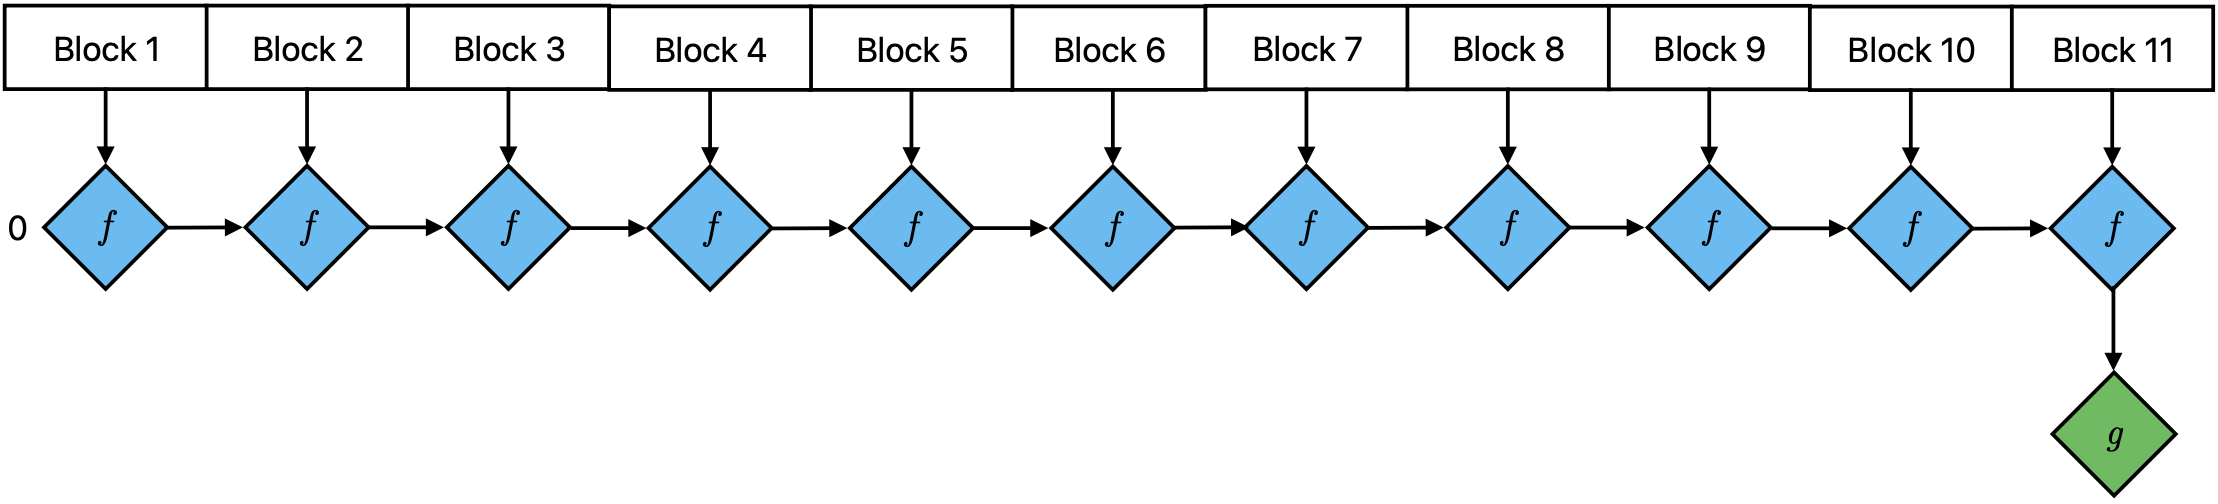
\includegraphics[width=1\textwidth]{linear-construction.png}
\caption{Merkle–Damgård Construction Overview}
\label{fig:linear-construction}
\end{figure}

\clearpage
\subsection{The Wide-Pipe Construction Variant} \label{widepipe}

The \textbf{Wide-Pipe} construction serves as a variant of the traditional Merkle–Damgård architecture and aims to improve the hash function's cryptographic resilience.\\\\
The standard Merkle–Damgård construction has been found vulnerable to certain types of cryptographic attacks, including length extension and multicollision attacks. The Wide-Pipe variant mitigates these vulnerabilities by modifying the hash function's internal state.
In this construction, the size of the internal state (\(s_b\)) is deliberately made much larger than the size of the hash output
(\(s_h\)), as expressed by the inequality:
\begin{align*}
    s_b \gg s_h
\end{align*}

This design choice serves to complicate potential attack vectors by introducing a greater level of computational complexity.
As a result, the hash function gains increased resistance against certain types of attacks that exploit the limitations of the Merkle–Damgård construction.\\\\
While performance remains our primary focus, the algorithm we examine in this paper incorporates the Wide-Pipe idea. By doing so, it offers a dual advantage: performance efficacy, which is central to this study, along with good cryptographic resilience, which is an undeniable advantage even in the realm of non-cryptographic hash functions.

\subsection{Other Variants}

While the classical Merkle–Damgård construction provides a reliable framework for cryptographic hash functions, there are a wide number of variants\cite{merkle_damgard_alternatives_review}. In this section, we discuss some of the most popular variants around opportunities for performance enhancement.

\subsubsection{Sponge Construction}

The Sponge construction,  proceeds in two phases: absorption and squeezing.
During the absorption phase, blocks of input data are XORed into a portion of the internal state, followed by a cryptographic permutation of the entire state. Importantly, each absorption step is inherently sequential, as it relies on the state resulting from the cryptographic permutation of the previous step. Consequently, the algorithm cannot benefit from instruction-level parallelism during the absorption phase.
The squeezing phase, which follows the absorption of all input blocks, generates the output hash from the internal state.
The opportunity for parallelization with the Sponge construction is thus constrained by its sequential nature during the absorbing phase.

\subsubsection{HAIFA Construction}

The HAsh Iterative FrAmework (HAIFA) not only mitigates vulnerabilities but also incorporates features like support for a configurable number of rounds and real-time incremental hashing.
However, like the standard Merkle–Damgård and Sponge constructions, the HAsh Iterative FrAmework (HAIFA) is also inherently sequential in its processing of message blocks.
Each iteration of the compression function in HAIFA depends on the outcome of the previous iteration.
This dependency chain means that the construction does not naturally lend itself to instruction-level parallelism (ILP), although other types of optimizations may still be possible depending on the specific implementation and hardware architecture.

\subsubsection{Tree Hashing}

Tree hashing breaks the input message into smaller fragments and processes them independently in a tree-like structure.
While tree-based hashing constructions offer a degree of parallelism, it is essential to recognize their inherent limitations. The extent of parallelization diminishes progressively as we move upward through the tree, owing to the dependencies between higher-level nodes. Here's a breakdown:

\begin{itemize}
\item \textbf{Leaf Level:} At this level, all blocks are independent, allowing the hashing operations to occur in parallel. If \( n \) is the number of leaves, then \( \frac{n}{2} \) parallel operations can occur for an even \( n \), or \( \frac{n-1}{2} + 1 \) for an odd \( n \).
\item \textbf{Second Level and Above:} The second level requires the hash results from the first level. Each node at the second level depends on two nodes from the level below, effectively halving the potential parallelism. This pattern of diminishing parallelization continues in subsequent levels.
\item \textbf{Final Level:} At the top of the tree, we are left with a single hash that relies on the two hashes beneath it. This operation is inherently sequential.
\end{itemize}

Although the tree-based hashing approach has a theoretical advantage in parallelization, practical implementations often face several challenges that can impact efficiency. These issues can make tree hashing hardly as efficient as a sequential structure for certain applications. Here are the primary factors:

\begin{itemize}
\item \textbf{Synchronization Overhead:} The parallel nature of the algorithm necessitates synchronization between different processing threads or units, especially at higher tree levels where dependencies exist. This overhead counters the gains from parallelization.
\item \textbf{Memory Consumption:} Tree constructions typically require more memory to store intermediate hash values, particularly when branching factors are high. Memory allocation and fragmentation usually impact performance.
\item \textbf{Cache Efficiency:} Unlike sequential algorithms that can benefit from cache locality, the tree-based approach often has to handle multiple non-contiguous data blocks, potentially leading to cache misses and reduced efficiency.
\item \textbf{Implementation Complexity:} The algorithmic and data-structure requirements for implementing tree-based hashing are more complex than those of a straightforward sequential hashing algorithm. The increased complexity can introduce more room for errors and maintenance challenges.
\end{itemize}

In light of these practical challenges, tree-based constructions might not be the best fit given our high-performance goals and the architecture of today's general-purpose computers.

\clearpage
\section{High ILP Construction} \label{highilp}

Most modern general-purpose CPUs employ a superscalar architecture which enables Instruction-Level Parallelism (ILP). 
Minimizing dependencies in an algorithm allows a superscalar processor to execute more instructions concurrently, thus maximizing its inherent parallelism and overall performance.
The key limitation for ILP in the Merkle–Damgård construction is the inherent sequential dependency: each block's hash depends on the result of hashing the previous block.

\subsection{ILP Awareness}

While compilers and CPUs employ various techniques to optimize ILP, their capabilities are often constrained by the inherent data dependencies in the code. It's for this reason that algorithmic design can be pivotal. By structuring algorithms to minimize dependency chains from the outset, we create opportunities for higher ILP that even the most advanced compiler optimizations and CPU features cannot achieve alone. Therefore, algorithmic design that is mindful of ILP can be a game-changer for performance optimization.

\subsubsection{Example}
Let's take a FNV-like hashing function. The "naive" way to process an array of elements would look like the \texttt{baseline} method, as shown in Rust snippet (Figure~\ref{fig:ilp_rust_example}). As we can see, every loop iteration requires the value of \texttt{h}, which has been computed the iteration before. Here we have a dependency chain, preventing the compiler from doing any optimization.

To make ILP possible, for the function \texttt{temp} we unroll the loop and hash a few inputs altogether, independently from \texttt{h}, and mix it once thereafter with \texttt{h}. We still have a dependency chain on \texttt{h}, but for fewer iterations.
The temporary hashes are independent and thus eligible for ILP.

Another track taken for the function \texttt{laned} is to unroll the loop and hash on separate lanes, and then mix the lanes together upon exiting the loop. Each lane has its own dependency chain but also on fewer iterations.

\begin{figure}[H]
\begin{multicols}{2}
\begin{lstlisting}[language=Rust, style=boxed]
const PRIME: u64 = 0x00000100000001b3;
const OFFSET: u64 = 0xcbf29ce484222325;

#[inline]
fn hash(hash: u64, value: u64) -> u64 {
    (hash ^ value) * PRIME
}

fn baseline(input: &[u64]) -> u64 {
    let mut h = OFFSET;
    let mut i: usize = 0;
    while i < input.len() {
        h = hash(h, input[i]);

        i = i + 1;
    }
    h
}

fn unrolled(input: &[u64]) -> u64 {
    let mut h: u64 = OFFSET;
    let mut i: usize = 0;
    while i < input.len() {
        h = hash(h, input[i]);
        h = hash(h, input[i + 1]);
        h = hash(h, input[i + 2]);
        h = hash(h, input[i + 3]);
        h = hash(h, input[i + 4]);

        i = i + 5;
    }
    h
}
\end{lstlisting}
\columnbreak
\begin{lstlisting}[language=Rust, style=boxed]
fn temp(input: &[u64]) -> u64 {
    let mut h: u64 = OFFSET;
    let mut i: usize = 0;
    while i < input.len() {
        let mut tmp: u64 = input[i];
        tmp = hash(tmp, input[i + 1]);
        tmp = hash(tmp, input[i + 2]);
        tmp = hash(tmp, input[i + 3]);
        tmp = hash(tmp, input[i + 4]);

        h = hash(h, tmp);

        i = i + 5;
    }
    h
}

fn laned(input: &[u64]) -> u64 {
    let mut h1: u64 = OFFSET;
    let mut h2: u64 = OFFSET;
    let mut h3: u64 = OFFSET;
    let mut h4: u64 = OFFSET;
    let mut h5: u64 = OFFSET; 
    let mut i: usize = 0;
    while i < input.len() {
        h1 = hash(h1, input[i]);
        h2 = hash(h2, input[i + 1]);
        h3 = hash(h3, input[i + 2]);
        h4 = hash(h4, input[i + 3]);
        h5 = hash(h5, input[i + 4]);

        i = i + 5;
    }
    hash(hash(hash(hash(h1, h2), h3), h4), h5)
}
\end{lstlisting}
\end{multicols}
\caption{FNV-like hash functions in Rust}
\label{fig:ilp_rust_example}
\end{figure}

\clearpage
\subsubsection{Benchmark}
Here are the timing on both an x86 and an ARM CPU. It also includes timing for the function \texttt{unrolled}, to show that performance increase comes indeed from ILP and not the loop unrolling itself.
We can see that \texttt{temp} and \texttt{laned} performed equally, leveraging ILP for a significant performance increase over the \texttt{baseline}.

\begin{figure}[H]
\centering
\begin{tabular}{|c|c|c|c|c|}
\hline
CPU & \texttt{baseline} & \texttt{unrolled} & \texttt{temp} & \texttt{laned} \\
\hline
AMD Ryzen 5 5625U (x86 64-bit) & 92.787 µs & 93.047 µs & 37.516 µs & 37.434 µs \\
Apple M1 Pro (ARM 64-bit) & 125.23 µs & 124.42 µs & 28.507 µs & 30.716 µs \\
\hline
\end{tabular}
\caption{Benchmark timings for ILP example}
\label{tab:your_table_label}
\end{figure}

While the \texttt{temp} and \texttt{laned} functions won't yield exactly the same hashes as the \texttt{baseline}, they serve the same purpose, while being much faster.
Both approaches have their pros and cons. As the \texttt{laned} explicitly declares \( n \) variables for our lanes, this approach is simpler in regards to compiler analysis and is thus more likely to benefit from ILP, regardless of the compiler or programming language used.
The following section will delve more in depth into the definition of a \textbf{Laned Construction}.

\clearpage
\subsection{The Laned Construction}

The \textbf{Laned Construction} introduces \( k_b \) lanes, and processes the message by groups of \( k_b \) blocks, so that for a given group each of the \( k_b \) block and be processed on its own lane. This way, we have \( k_b \) independent dependency chains. The lane hashes can then be compressed altogether thereafter upon exiting the loop.

\subsubsection{Intermediate Hashes}

Let's define \( n_g = \lfloor {n_b}/{k_b} \rfloor \) as the number of whole groups of \( k_b \) message blocks. \\
For each lane we compute an intermediate hash, \( H_i \), as follows:

\begin{align*}
H_{1} &= f(\ldots f(f(f(0^{s_b}, M_{0k_b + 1}), M_{1k_b + 1}), M_{2k_b + 1})\ldots, M_{n_g + 1}) \\
H_{2} &= f(\ldots f(f(f(0^{s_b}, M_{0k_b + 2}), M_{1k_b + 2}), M_{2k_b + 2})\ldots, M_{n_g + 2}) \\
&\vdots \\
H_{k_b} &= f(\ldots f(f(f(0^{s_b}, M_{0k_b + k_b}), M_{1k_b + k_b}), M_{2k_b + k_b})\ldots, M_{n_g + k_b}) \\
\end{align*}

\subsubsection{Final Hash}

The final hash \( H \) is calculated using \( f \) to compress the intermediate hashes and the remaining message blocks (if any),
which is then passed through \( g \):

\begin{equation*}
h(M) = g\left( f( \ldots f(f(\ldots f(f(0^{s_b}, H_1), H_2) \ldots, H_{k_b}), M_{{k_b}{n_g}+1}) \ldots, M_{n_b} ) \right).
\end{equation*}

\begin{figure}[H]
\centering
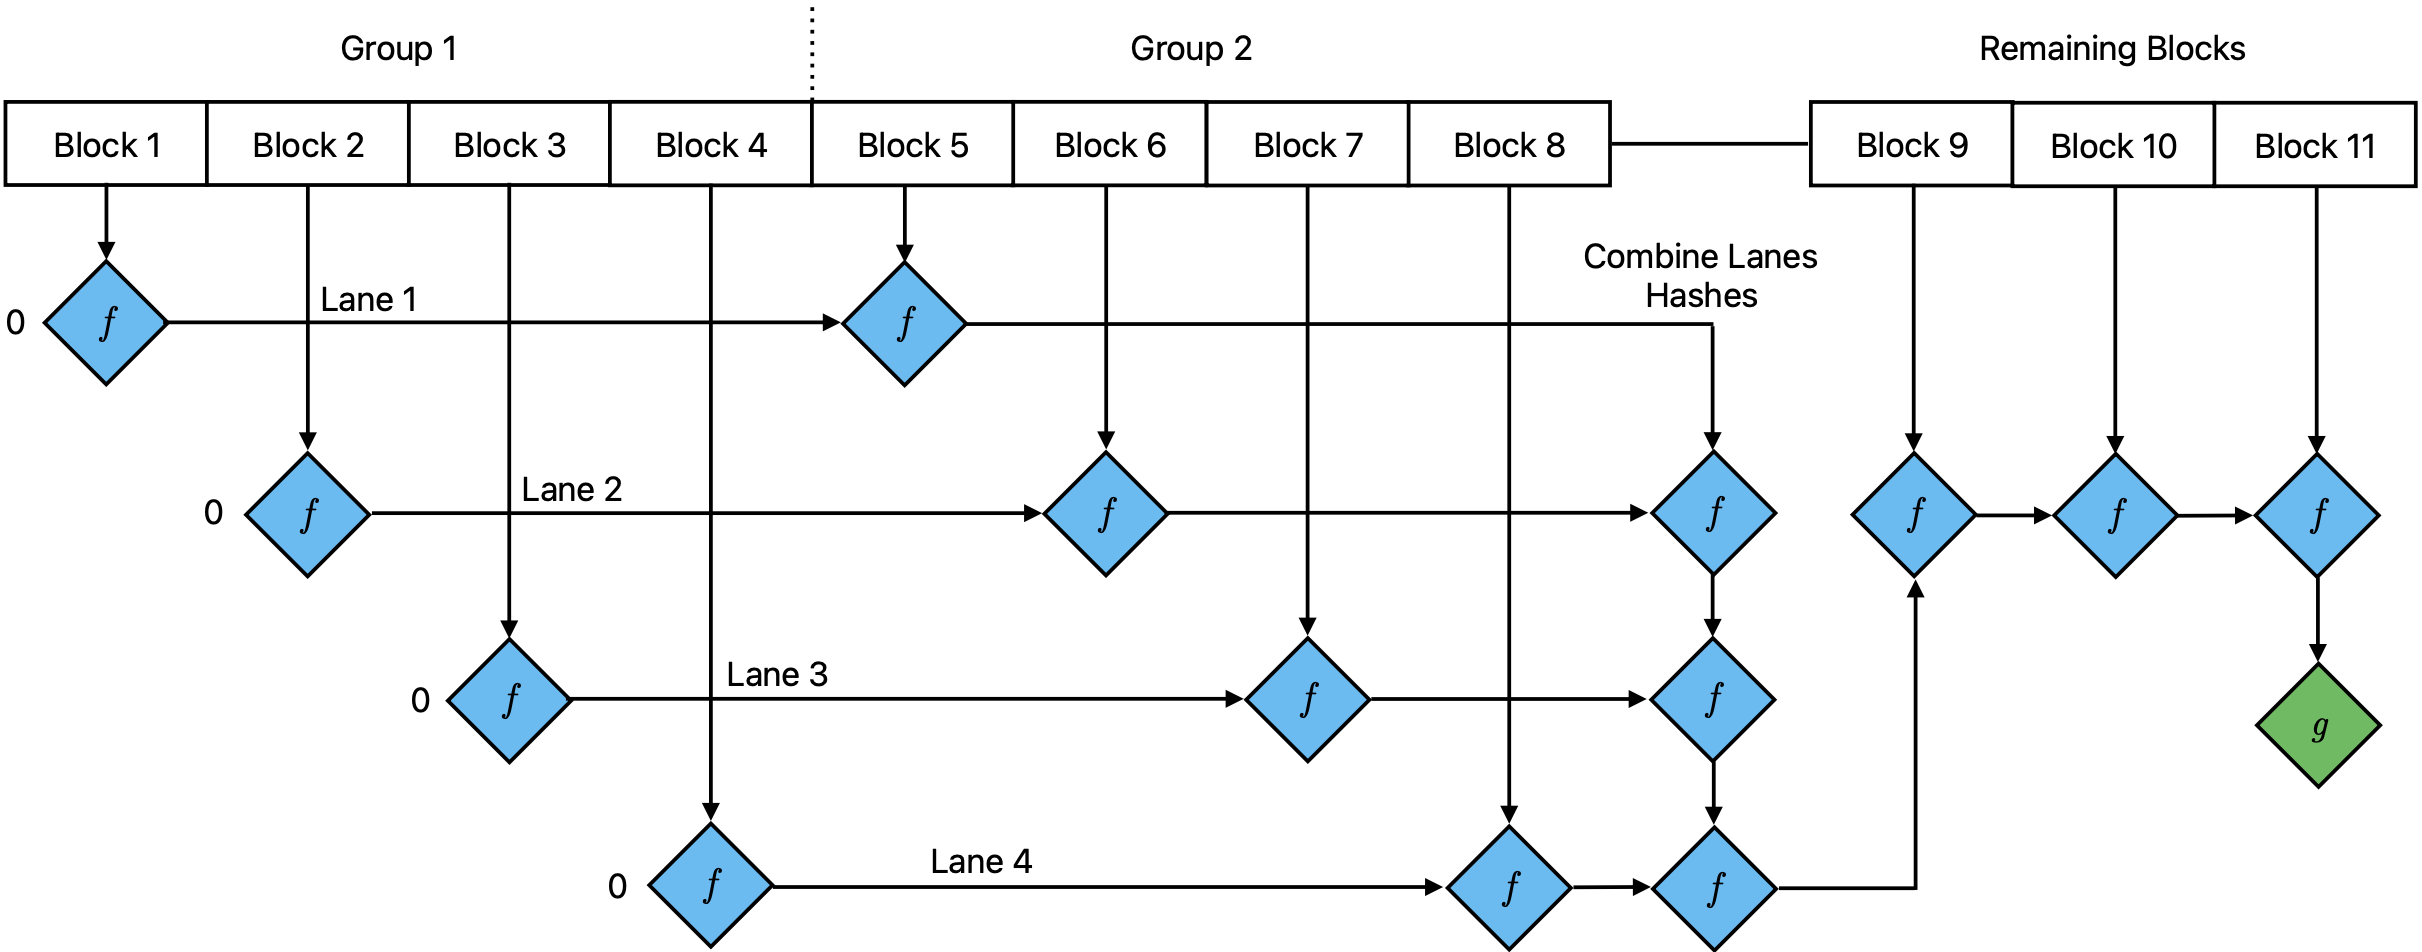
\includegraphics[width=1\textwidth]{laned-construction.png}
\caption{Laned Construction Overview}
\label{fig:linear-construction}
\end{figure}

An alternative to chaining usages of \( f \) is to compress lane hashes by pair, and subsequently compressing the resulting hashes also by pair until we are left with a single hash (for instance \(f(f(f(H_1, H_2), f(H_3, H_4)), f(...))\)). In practice, this would allow some form of ILP on the final hash composition as well, decreasing as we get closer to the final hash.

\clearpage
\section{The GxHash Algorithm}

The \textbf{GxHash} hashing algorithm is designed to maximize throughput by optimizing for Instruction-Level Parallelism (ILP) and making extensive use of Single Instruction, Multiple Data (SIMD) instructions. Notably, while these optimization avenues are orthogonal — focusing on parallelized and vectorized instructions respectively — they collectively harness the full potential of modern CPU architectures.\\\\
This design philosophy introduces specific constraints for the compression and finalization functions:

\begin{itemize}
    \item \textbf{Utilization of Hardware Intrinsics:} To achieve the SIMD-oriented goal, arithmetic operations are tailored to be compatible with both x86 and ARM Neon intrinsics.
    \item \textbf{Efficiency through Simplicity:} Minimizing the number of operations is crucial, as fewer operations typically translate to faster execution.
    \item \textbf{Hash Quality Assurance:} Despite these performance optimizations, the algorithm must ensure a minimum level of hash quality to maintain low collision probabilities.
\end{itemize}

In the next sections, we'll delve into the specific operations and transformations chosen for the compression and finalization functions of the \textbf{GxHash} algorithm (version 1.0.0).

\subsection{Pipe Width}

To optimize throughput, the pipe width \( s_b \) is set to match the native width of the CPU's SIMD registers.
This alignment ensures that each SIMD instruction operates on the entire pipe width, maximizing data processed per instruction.
Given that typical SIMD registers are at least 128 bits in width, the pipe width surpasses common 32-bit or 64-bit output hash sizes.
Consequently, the GxHash design aligns with the characteristics of a wide-pipe construction, as discussed in section \ref{widepipe}.
This makes GxHash more resistant to multicollision attacks.

\subsection{Compression}

The role of the compression function is to transform a larger input (or message) into a smaller, fixed-size output. Due to this inherent reduction in size, the compression function cannot be bijective.

To delve deeper into this, consider the definition of a bijective function. A function is bijective if and only if it is both injective (one-to-one) and surjective (onto). In simpler terms, for every unique input, there is a unique output, and every possible output has a corresponding input.

Given the nature of the compression function \( f: \{0,1\}^{s_b} \times \{0,1\}^{s_b} \to \{0,1\}^{s_b} \), where the domain is much larger than the codomain (\( s_b \times s_b > s_b \)), it becomes mathematically impossible for the function to be one-to-one. There will inevitably be multiple different inputs that map to the same output, known as collisions.\\

With the inevitable non-bijectivity, the performance requirements and the limited set of available SIMD intrinsics, the selection for the compression has to be empirical, thus implying specifying a version to account for these current choices that may be improved in future versions.\\

TODO
In practice, the \textbf{GxHash} uses the AES block cipher intrinsics to combines two 128-bit SIMD vectors together combination of SIMD 8-bit wrapping add and state-wide circular shift of one. The addition is a simple way to mix the state with the next message block bits, while providing an arithmetic carry which helps in regard to distribution (as opposed to a XOR for instance). Adding on a 8-bit basis also helps in regards to distribution, as opposed to adding on larger bit widths. This operation alone however comes with several weaknesses:
\begin{itemize}
\item Such a simple operation is inherently weak to different kind of attacks. This can however be partially addressed with a more robust bit mixing for the finalization function. In the context of non-cryptographic hashing, which is the scope of usage of our algorithm, we think it is an acceptable compromise.
\item A major issue lies in the addition being associative (\(a \cdot b) \cdot c = a \cdot (b \cdot c \)). An associative compression function would make the hashing algorithm insensitive to the ordering of the input message blocks, which is something we want to avoid. To address this, we circularly shift the state bits by one.
\end{itemize}

\begin{figure}[H]
\begin{multicols}{2}
\begin{lstlisting}[language=Rust, style=boxed]
// For ARM 64-bit

use core::arch::aarch64::*;

pub fn compress(a: int8x16_t, b: int8x16_t)
-> int8x16_t {
    let sum: int8x16_t = vaddq_s8(a, b);
    return vextq_s8(sum, sum, 1);
}
\end{lstlisting}
\columnbreak
\begin{lstlisting}[language=Rust, style=boxed]
// For x86 64-bit

use core::arch::x86_64::*;

pub fn compress(a: __m256i, b: __m256i)
-> __m256i {
    let sum: state = _mm256_add_epi8(a, b);
    return _mm256_alignr_epi8(sum, sum, 1);
}
\end{lstlisting}
\end{multicols}
\caption{GxHash Compression in Rust}
\label{fig:compression_rust_example}
\end{figure}

\subsection{Finalization}

The finalization process in the GxHash algorithm is crucial to ensure the transformation of its internal state into a fixed-size, uniformly distributed hash output. This process is delineated into two primary steps: mixing the bits and reducing to the desired hash size.

This mixing step is responsible for ensuring the even distribution of bits in the state, thereby reducing patterns or biases that might arise from the input data or the compression process. Given the inherent simplicity of the GxHash compression, it is worth for the finalization to incorporate slightly more intricate bit mixing operations, especially given it runs only once per message hashed, as opposed to the compression that occurs once for each block.\\
Leveraging SIMD capabilities can help in regard to performance and efficiency, which remains for us a primary consideration. Fortunately, both x86 and ARM architectures provide AES (Advanced Encryption Standard) intrinsics that serve as efficient tools for bit mixing. The use of three AES block cipher rounds ensures a robust diffusion of bits across the state at a cheap computational cost.\\
The AES keys can be set changed, providing a way to have unique hashes per-application and even per-process, protecting from eventual precomputed or replay attack attempts.

Once the state's bits have been thoroughly mixed, the next step is to reduce this state into a smaller, fixed-size hash output, typically 32 or 64 bits. There are several approaches to this, one being combiniting the \( X \)-bit integer parts of the mixed state together (by xoring them together for instance). GxHash takes a simpler path by reinterpreting our state into a smaller \( X \)-bit value, assuming an uniform distribution at the mixing stage thanks to the 3 rounds of AES. This allow the GxHash algorithm to generate hashes of any size up to \( s_b \) bits with virtually no additional computational cost.

\subsection{Implementation Details}

\subsubsection{CPU Alignement}

Data alignment in memory, commonly referred to as CPU alignment, directly impacts the efficiency of data access and processing. The CPU is optimized to access data from addresses that align with its natural word size. When data is properly aligned, the CPU can retrieve and process it in fewer cycles, resulting in increased computational efficiency.

In practice, programs typically allocate memory with alignment, ensuring data is generally aligned. However, a given input message to our hash function is still not guaranteed to be aligned. To handle this case, we can either read our data with an offset to account for the misalignment (at the cost of a much-increased complexity) or use specific SIMD intrinsics designed to handle potentially unaligned data. 

Benchmarks conducted show a less than 20\% performance degradation on both our x86 and ARM hardware when using the second solution. For simplicity, GxHash treats aligned and unaligned data the same way.

\subsubsection{Low-Overhead Looping}

While the looping semantics will vary from one language to another, any overhead from looping over the input message blocks is likely to directly affect the overall throughput of the algorithm, given how optimized the rest of the algorithm is meant to be. In some cases, compilers might do a great job at generating loop instructions with minimal overhead, but it isn't the case in the language where GxHash was ported, where looping using pointer arithmetics was needed.

Unrolling the loop is a complementary optimization that diminishes greatly any loop overhead. In the case of GxHash, the temporal construction implies some kind of unrolling, which is sufficient for achieving the high throughput numbers we see in our benchmarks.

\subsubsection{Padding}

\textbf{Merkle–Damgård} and derivatives can handle message of an arbitrary size \( s_m \) by padding the message upfront with the padding function \( p: \{0,1\}^{s_m} \to \{0,1\}^{n_b \times s_b} \) where \( n_b = \lceil s_m/s_b \rceil \). In the case where the last block is not whole, the padding fills it with zero-bytes until the size \( s_b \) is reached. The last block can then be processed like any other block by the compression function.

In practice, a naive implementation for \( p \) for GxHash in computer code implies copying the remaining bytes into a zero-initialized buffer of size \( s_b \), which can then be loaded onto an SIMD registry and then handed to the compression. In our performance-critical context, these allocations and copies introduce significant overhead.

\paragraph{Read Beyond and Mask}\leavevmode\\
To avoid this overhead, one possible trick consists of reading \( s_b \) bytes starting from the last block address, even if it implies reading beyond the memory storing the input message. The read bytes can then be masked with the help of a sliding mask, transforming the trailing bytes that don't belong to our message into zeros, in a single SIMD operation. Compared to the naive method, this solution is up to ten times faster on our test machine (Ryzen 5, x86 64-bit).

\begin{figure}[H]
\begin{lstlisting}[language=Rust, style=boxed]
use core::arch::x86_64::*;

unsafe fn read_padded(p: *const __m128i, len: isize) -> __m128i {
    // Consecuive indices on which we compare the length against, byte per byte, to retreive our mask.
    // The order is descending or ascending depending on the endianness
    let indices = _mm_set_epi8(15, 14, 13, 12, 11, 10, 9, 8, 7, 6, 5, 4, 3, 2, 1, 0);
    // Computing the mask
    let mask = _mm_cmpgt_epi8(_mm_set1_epi8(len as i8), indices);
    // Read beyond and mask
    partial_vector = _mm_and_si128(_mm_loadu_si128(p), mask);
}
\end{lstlisting}
\caption{GxHash Padding in Rust}
\label{fig:read_beyond_example}
\end{figure}

\paragraph{Safety Considerations}\leavevmode\\
Reading beyond a specified pointer might access memory not mapped to the program's address space or that's protected. If the program tries to read this memory, the OS detects the violation, typically causing a crash. This mechanism ensures processes don't interfere with each other or access critical memory areas. Although rare, the potential for this issue exists.

In modern computers, memory is divided into chunks called pages. A program can access any part of its assigned page without system-level errors like segmentation faults. We can check if an unsafe operation is within a single page. If it is, we can use the optimized method; if not, we fallback to the naive method.

Memory pages are designed so addresses within them share higher bits and vary only in lower bits, representing offsets. The code in figure~\ref{fig:check_page_example} uses this principle, considering a page size of 4096. The likelihood of having 32 bytes on the same page exceeds 99\%. This safety check is cost-effective, retaining most performance benefits while ensuring safety.

\begin{figure}[H]
\begin{lstlisting}[language=Rust, style=boxed]
unsafe fn is_same_page(ptr: *const __m128i) -> bool {
    // Usual minimal page size on modern computers
    const PAGE_SIZE = 4096;
    // Get the actual pointer address integer value
    let address = ptr as usize;
    // Mask to keep only the last 12 bits (2^12 = 4096)
    let offset_within_page = address & 0xFFF;
    // Check if the 16th byte from the current offset exceeds the page boundary
    offset_within_page <= (PAGE_SIZE - 31)
}
\end{lstlisting}
\caption{Read-Beyond Safety Check in Rust}
\label{fig:check_page_example}
\end{figure}

\clearpage
\section{Benchmarks}

\subsection{Quality}

\subsubsection{Benchmark Quality Criteria}
The primary quality criteria for non-cryptographic hash functions include:

\begin{itemize}
    \item \textbf{Uniform Distribution:} A high-quality hash function distributes its output values as uniformly as possible across the output space. This ensures that, when used in applications like hash tables, the data is spread evenly, reducing clustering and the frequency of collisions.

    We can estimate the uniformity of the distribution by counting the number of times each bit is set and computing a standard deviation. This "bit distribution" criteria however does not qualify the distribution of the hashes as a whole, so a complementary estimator is the "bucketed distribution", which be computed by placing generated hashes into a fixed-size grid and counting occurrences. This can also be easily displayed as a bitmap as a convenient way to visualize distribution.
    \item \textbf{Minimal Collisions:} While no hash function can be entirely collision-free due to the pigeonhole principle, a good non-cryptographic hash should minimize collisions for typical input sets, ensuring that different inputs usually produce distinct outputs.
    
    The collision rate can be computed by counting unique values with the help of an hash table.
    \item \textbf{Avalanche Effect:} A subtle change in the input should result in a considerably different output, ensuring sensitivity to input variations. This also contributes to lessening the risk of clustered hashes in applications like hash tables.
    
    The avalanche effect can be computed by flipping a single random bit for a given input and checking the differences between the hashes generated before and after the bit was flipped. Ideally, half of the bit should change on average.
    \item \textbf{Performance:} The performance of a noncryptographic hash function is usually reflected by the performance of the application using it. For instance, a fast non-cryptographic hash function generally implies a fast hash table. This specific criteria will be tackled in the next section which is dedicated to it. 

\end{itemize}

\subsubsection{Quality Results}

While we can compute quality metrics, the result will greatly vary depending on the actual inputs used for our hash function. Let's see how the GxHash algorithm qualifies in specific scenarios against some well-known non-cryptographic algorithms, such as:

\begin{itemize}
\item \textbf{HighwayHash}\cite{highwayhash} The latest non-cryptographic hash algorithm from Google Research
\item \textbf{xxHash}\cite{xxhash} Recently a very popular algorithm for fast non-cryptographic hashing
\item \textbf{t1ha0}\cite{rust-t1ha} Supposedly the fastest algorithm at the time of writing
\end{itemize}

\clearpage
\paragraph{Random Blobs}\leavevmode\\
For the first scenario, we randomly generate 1,000,000 inputs of size 4 bytes, 64 and 1000 to observe how the hash function behaves with truly unpredictable data, and for different input sizes.

\begin{table}[H]
\centering
\begin{tabular}{|l|r|r|r|r|}
\hline
\textbf{Function for Random dataset} & \textbf{Collisions} & \textbf{Bits Distribution} & \textbf{Distribution} & \textbf{Avalanche} \\
\hline
UInt32 GxHash(4)            & 0,0241\% & 0,001094  & 0,000002 & 0,00034 \\
UInt32 GxHash(64)           & 0,0115\% & 0,000795  & 0,000002 & 0,00002 \\
UInt32 GxHash(1000)         & 0,0108\%  & 0,001007  & 0,000002 & 0,00007 \\
UInt32 HighwayHash(4)        & 0,0237\% & 0,001135  & 0,000002 & 0,00001 \\
UInt32 HighwayHash(64)       & 0,0117\% & 0,001028  & 0,000002 & 0,00078 \\
UInt32 HighwayHash(1000)     & 0,0103\% & 0,00092   & 0,000002 & 0,00032 \\
UInt32 T1ha(4)               & 0,021\%  & 0,001034  & 0,000002 & 0,00002 \\
UInt32 T1ha(64)              & 0,0123\% & 0,000933  & 0,000002 & 0,00047 \\
UInt32 T1ha(1000)            & 0,0114\% & 0,001087  & 0,000002 & 0,00027 \\
UInt32 XxHash(4)            & 0,0119\% & 0,00102   & 0,000002 & 0,00027 \\
UInt32 XxHash(64)           & 0,013\%  & 0,000871  & 0,000002 & 0,00083 \\
UInt32 XxHash(1000)         & 0,0131\% & 0,001214  & 0,000002 & 0,00038 \\
UInt32 Fnv1a(4)             & 0,031\%  & 0,001008  & 0,000002 & \textcolor{red}{0,20155} \\
UInt32 Fnv1a(64)            & 0,0094\% & 0,000748  & 0,000002 & \textcolor{orange}{0,08599} \\
UInt32 Fnv1a(1000)          & 0,0138\% & 0,000821  & 0,000002 & \textcolor{orange}{0,07861} \\
UInt32 Crc(4)               & 0,0119\% & 0,000811  & 0,000002 & \textcolor{red}{0,11689} \\
UInt32 Crc(64)              & 0,0117\% & 0,001041  & 0,000002 & \textcolor{orange}{0,02473} \\
UInt32 Crc(1000)            & 0,0123\% & 0,001097  & 0,000002 & 0,00514 \\
\hline
\end{tabular}
\caption{Quality benchmark results for the random dataset at 1,000,000 iterations}
\label{tab:quality-data-random}
\end{table}
    
All numbers are very low, and GxHash quality results are of the same order of magnitude as for other algorithms. Distribution is very good for all algorithms. Avalanche is good for most algorithms, except for FNV-1a and CRC. We can notice that avalanche score for GxHash is an order of magnitude better than other algorithms for larger input sizes.

We can notice a collision rate of about 0.011\% and even 0.022\% for the 4 bytes inputs. There is an explanation: we can derive from the birthday paradox problem the following formula to estimate the \% of collisions:

\begin{align*}
    100 \times \frac{n^2}{2 \times m \times n}
\end{align*}

Where \(n\) is the number of samples and \(m\) is the number of possible values. When \(n=1000000\) and \(m=2^{32}\) we obtain 0.0116\%.
You can see that this value closely matches most of the collision rates benchmarked. This is because the generated hashes are of 32-bit size,
thus naturally colliding at this rate. For inputs of size 4, the inputs themselves are also likely to collide with the same odds (because inputs are randomly generated). For this reason, the collision rate is expected to be about 2 \(\times\) 0.0116\%.
We can see however that CRC and XxHash\cite{xxhash} have lower odds of collisions for 4 bytes input, which can be explained by a size-specific logic to handle small inputs bijectively.

\begin{figure}[H]
\centering
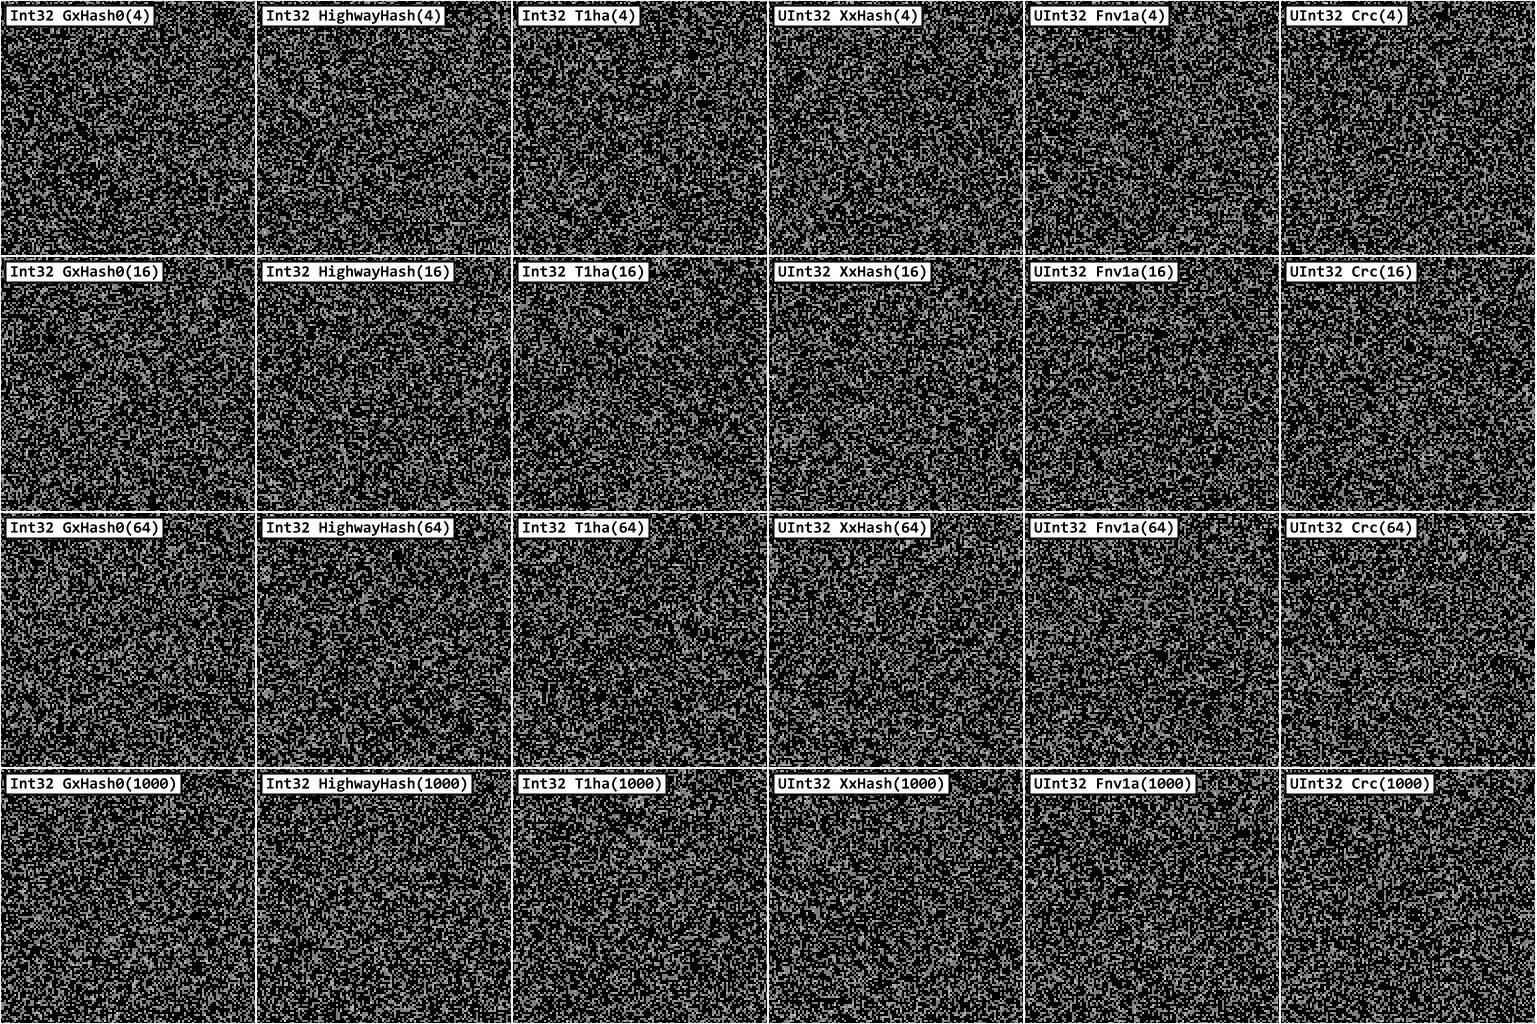
\includegraphics[width=1\textwidth]{quality-random.png}
\caption{Distribution map for random dataset}
\label{fig:quality-random}
\end{figure}

Here is a visualization of the distribution represented by bitmap, which each pixel being a bucket for generated hashes to fill. A black pixel is an empty pixel, and the whiter a pixel is the fuller of hashes the bucket is. 

We can see that all algorithms benchmarked have similar output in the case of random inputs, which is similar to noise noise. The lack of visible frequencies or "patterns" is a sign of good distribution. At a glance, we can see that all algorithm benchmarks have a good distribution for this dataset.

\clearpage
\paragraph{Sequential Numbers}\leavevmode\\
For the second scenario, we generate consecutive integers as inputs to observe how the function handles closely related values. Typically, close values could highlight potential weaknesses in distribution. We still run a number of 1,000,000 iterations, meaning that inputs will be integers from 1 to 1,000,000. Consequently, input bytes after the 4th will always remain 0, even for larger inputs. This can also be a challenge for a hash algorithm to keep entropy from the first few bytes of the input despite having to process many 0-bytes afterward.

\begin{table}[H]
\centering
\begin{tabular}{|l|r|r|r|r|}
\hline
\textbf{Function for Sequential dataset} & \textbf{Collisions} & \textbf{Bits Distribution} & \textbf{Distribution} & \textbf{Avalanche} \\
\hline
UInt32 GxHash(4)                & 0,013\% & 0,001132  & 0,000002 & 0,00044 \\
UInt32 GxHash(64)               & 0,0112\% & 0,000651  & 0,0000019 & 0,00039 \\
UInt32 GxHash(1000)             & 0,0126\% & 0,000818  & 0,000002 & 0,00029 \\
UInt32 HighwayHash(4)            & 0,0117\% & 0,00112   & 0,000002 & 0,00011 \\
UInt32 HighwayHash(64)           & 0,0104\% & 0,001204  & 0,000002 & 0,00044 \\
UInt32 HighwayHash(1000)         & 0,0112\% & 0,001188  & 0,000002 & 0,00131 \\
UInt32 T1ha(4)                   & 0,012\%  & 0,000746  & 0,000002 & 0,00076 \\
UInt32 T1ha(64)                  & 0,0125\% & 0,000987  & 0,000002 & 0,00071 \\
UInt32 T1ha(1000)                & 0,0113\% & 0,000944  & 0,000002 & 0,00003 \\
UInt32 XxHash(4)                & 0\%      & 0,000933  & 0,000002 & 0,00018 \\
UInt32 XxHash(64)               & 0\%      & 0,000907  & 0,000002 & 0,00046 \\
UInt32 XxHash(1000)             & 0\%      & 0,001081  & 0,000002 & 0,0007 \\
UInt32 Fnv1a(4)                 & 0\%      & 0,00009   & 0,0000017 & \textcolor{red}{0,18255} \\
UInt32 Fnv1a(64)                & 0\%      & 0,000064  & 0,0000022 & \textcolor{orange}{0,08281} \\
UInt32 Fnv1a(1000)              & 0\%      & 0,000042  & 0,0000018 & \textcolor{orange}{0,08416} \\
UInt32 Crc(4)                   & 0\%      & 0,000003  & 0,000002 & \textcolor{red}{0,11729} \\
UInt32 Crc(64)                  & 0\%      & 0,000003  & 0,0000004 & \textcolor{orange}{0,02542} \\
UInt32 Crc(1000)                & 0\%      & 0,00001   & 0,0000004 & 0,0046 \\
\hline
\end{tabular}
\caption{Quality benchmark results for the sequential dataset at 1,000,000 iterations}
\label{tab:my_label}
\end{table}

We still observe about 0.0116\% of collisions, which is still expected given the size of the hashes generated and the number of iterations. We can notice however that a few algorithms have managed to have 0 collisions. This is an interesting feature but nevertheless anecdotical: as inputs of this dataset may only have at most the four first bytes different than zero, some algorithms are able to keep the possible bijectivity.

TODO
Regarding distribution, we can notice that GxHash outperforms HighwayHash\cite{highwayhash}, XxHash\cite{xxhash} and T1ha0\cite{rust-t1ha}. Avalanche is slightly worse, however, possibly due to the tradeoff of doing fewer operations for greater performances. Overall, the numbers are all still very low and remain in the same ballpark, except for FNV-1a and CRC which still suffer from a relatively "high" avalanche.

\begin{figure}[H]
\centering
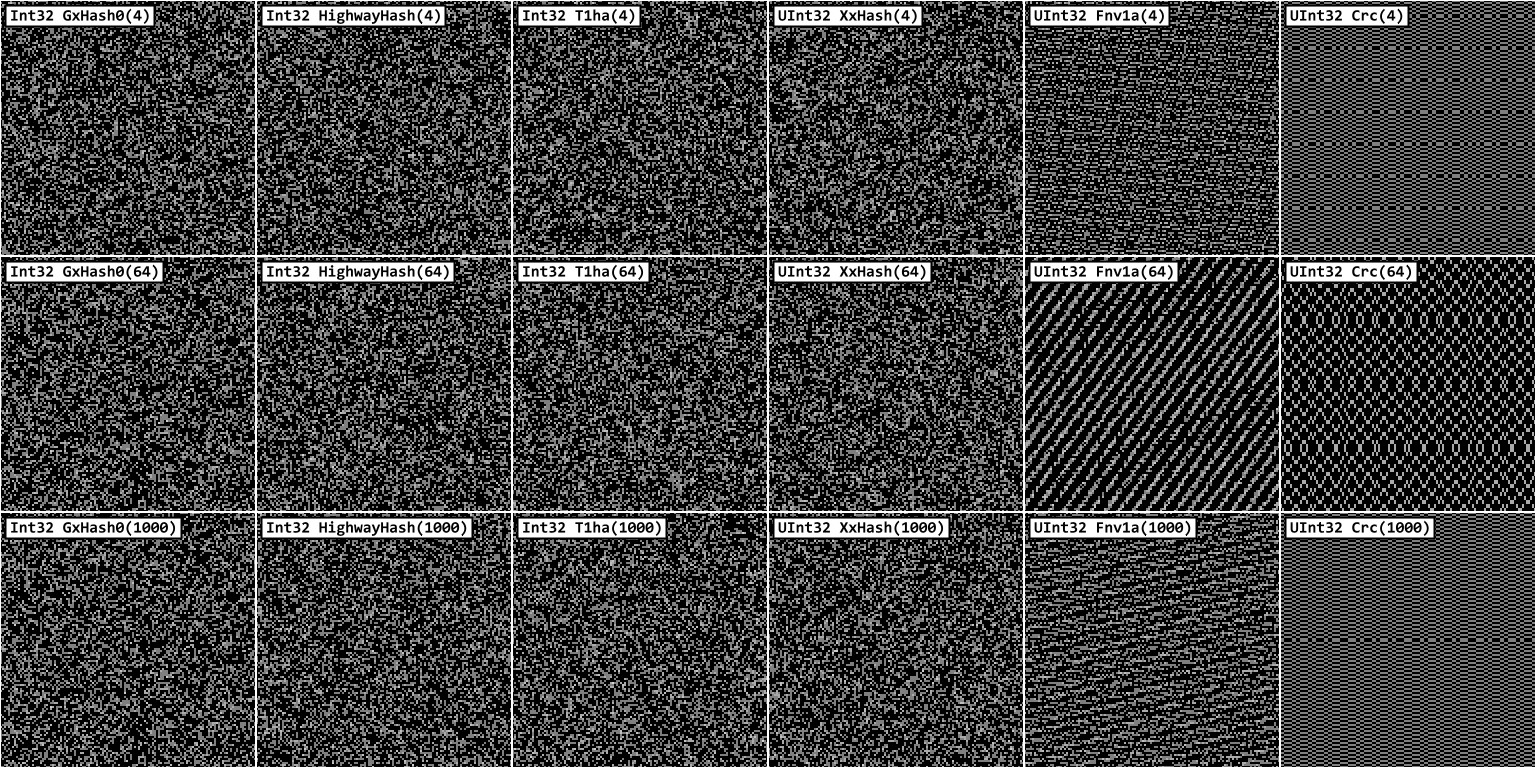
\includegraphics[width=1\textwidth]{quality-sequential.png}
\caption{Distribution map for sequential dataset}
\label{fig:quality-sequential}
\end{figure}

The distribution map is more interesting for sequential inputs. As a matter of fact, we clearly identify distribution patterns for FNV-1a and CRC. It isn't necessarily a bad thing, because a hash function can distribute the hash in a way that the distribution map looks evenly distributed (such as what we observe with CRC with 1000-bytes long inputs), however it implies that values hashes are correlated in a way, which a property we prefer to avoid for a non-cryptographic hash function. GxHash performs well in that matter, with a distribution that looks as uniform and uncorrelated than its counterparts HighwayHash\cite{highwayhash}, XxHash\cite{xxhash} and T1ha0\cite{rust-t1ha}.

\clearpage
\paragraph{English Words}\leavevmode\\
For the third scenario, we generate English-looking words as inputs by deriving a set of "real" English words with Markov chains to be able to generate many unique strings for any size. This allows us to observe how the function behaves in a close to "real-world scenario". We ignore on-purpose inputs of size 4 since we are not able to generate enough unique strings for that size.

\begin{table}[H]
\centering
\begin{tabular}{|l|r|r|r|r|}
\hline
\textbf{Function for MarkovWords dataset} & \textbf{Collisions} & \textbf{Bits Distribution} & \textbf{Distribution} & \textbf{Avalanche} \\
\hline
UInt32 GxHash(64)                & 0,0108\% & 0,00122  & 0,000002 & 0,00044 \\
UInt32 GxHash(1000)              & 0,0121\% & 0,001106  & 0,000002 & 0,00035 \\
UInt32 HighwayHash(64)            & 0,0123\% & 0,000809  & 0,000002 & 0,00048 \\
UInt32 HighwayHash(1000)          & 0,0117\% & 0,00092   & 0,000002 & 0,00078 \\
UInt32 T1ha(64)                   & 0,0111\% & 0,000803  & 0,000002 & 0,00064 \\
UInt32 T1ha(1000)                 & 0,0123\% & 0,001175  & 0,000002 & 0,00135 \\
UInt32 XxHash(64)                & 0,0106\% & 0,000766  & 0,000002 & 0,00046 \\
UInt32 XxHash(1000)              & 0,01\%   & 0,000892  & 0,000002 & 0,00021 \\
UInt32 Fnv1a(64)                 & 0,0122\% & 0,000998  & 0,000002 & \textcolor{orange}{0,08585} \\
UInt32 Fnv1a(1000)               & 0,0127\% & 0,000993  & 0,000002 & \textcolor{orange}{0,08143} \\
UInt32 Crc(64)                   & 0,0124\% & 0,000965  & 0,000002 & \textcolor{orange}{0,02467} \\
UInt32 Crc(1000)                 & 0,0123\% & 0,000708  & 0,000002 & 0,00499 \\
\hline
\end{tabular}
\caption{Quality benchmark results for words dataset at 1,000,000 iterations}
\label{tab:my_label}
\end{table}

We still observe about 0.0116\% of collisions for all algorithms, explainable by the birthday paradox as seen previously. This time however, XxHash\cite{xxhash}, Fnv1a and Crc are not able to beep bijectivity as inputs use more bytes compared to the sequential case, making the bijectivity property impossible and thus leading to inevitable collision.
The bits distribution is very close for all algorithms benchmarked, at about 0.001. The avalanche score for GxHash is very good, on pair with HighwayHash\cite{highwayhash}, XxHash\cite{xxhash} and T1ha\cite{rust-t1ha}.

\begin{figure}[H]
\centering
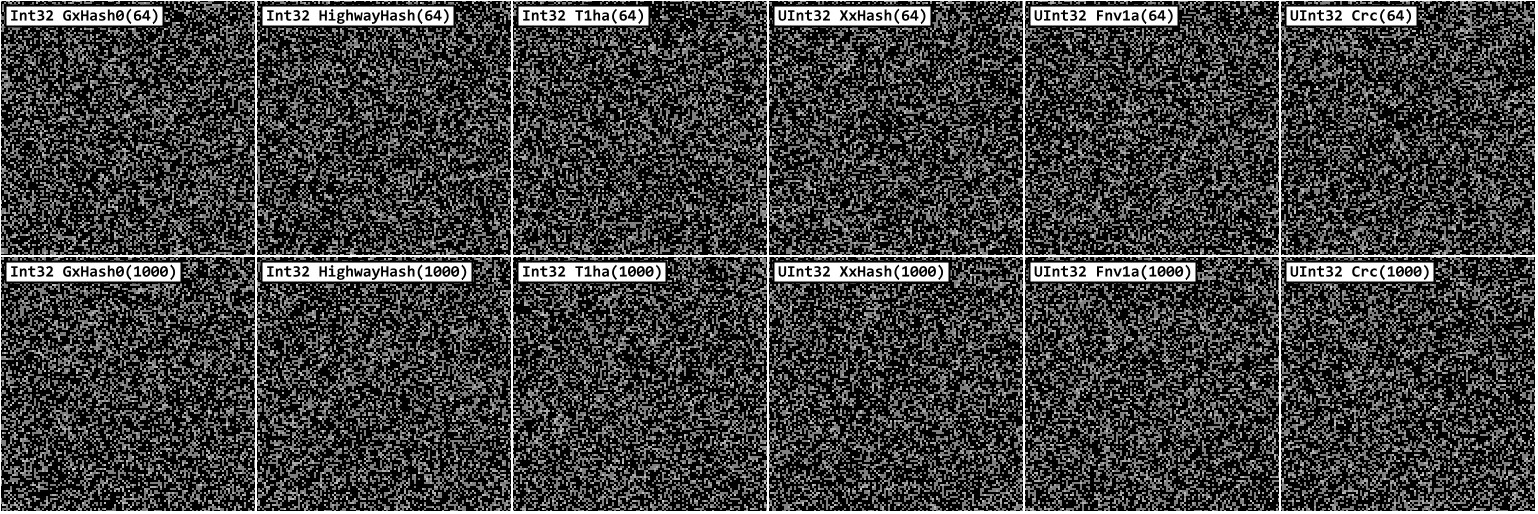
\includegraphics[width=1\textwidth]{quality-markov.png}
\caption{Distribution map for words dataset}
\label{fig:quality-sequential}
\end{figure}

Bucketed distribution is looking good in all cases for the English words case.

\subsubsection{Conclusion}

This was just an overview of the quality of the hashes produced by GxHash and a few comparisons to some established non-cryptographic algorithms. 

Our results demonstrate promising quality characteristics of GxHash with low collisions, good distribution, and a high avalanche effect, and its quality is comparable to other well-established non-cryptographic algorithms. However, it is essential to acknowledge the limitations of the presented evaluation scenarios. The benchmarks presented herein, namely random inputs, sequential inputs, and English word inputs, offer a glimpse into the algorithm's quality but are by no means exhaustive. In real-world applications, the behavior of a hash algorithm can be influenced by a myriad of factors and specific data patterns. As such, while our findings provide a foundational understanding of GxHash's quality, potential users should be cognizant that results may vary based on the actual use case and the nature of the input data.

\clearpage
\subsection{Performance}

Performance is measured as a throughput, in gibibytes of data hashed per second (higher is better). This is a common measurement unit for performance in this field. Performance is measured against inputs of size 4, 16, 64, 246, 1024, 4096 and 16384 to cover a broad range of use cases.

For reference, we'll also benchmark other non-cryptographic algorithms under the same conditions, thanks to their Rust implementations, namely: t1ha\cite{rust-t1ha}, xxhash\cite{twox-hash} and HighwayHash\cite{highway-rs}.

The benchmark is run on three different setups:
\begin{itemize}
    \item A Ryzen 5 equipped low-budget desktop PC
    \item An n2-standard-2 compute GCP virtual machine (likely equipped with an Intel Xeon 8376H). Cloud computing is very popular nowadays and the hardware is quite different from the desktop PC.
    \item A Macbook Pro with an M1 Pro chip, to test the algorithm on an ARM architecture which implies different SIMD intrinsics and likely different performance results. Note that the T1ha-0 implementation benchmarked does not leverage ARM intrinsics, and this is why it is not benchmarked for this platform (the portable version would perform too poorly).
\end{itemize}

\begin{figure}[H]
\centering
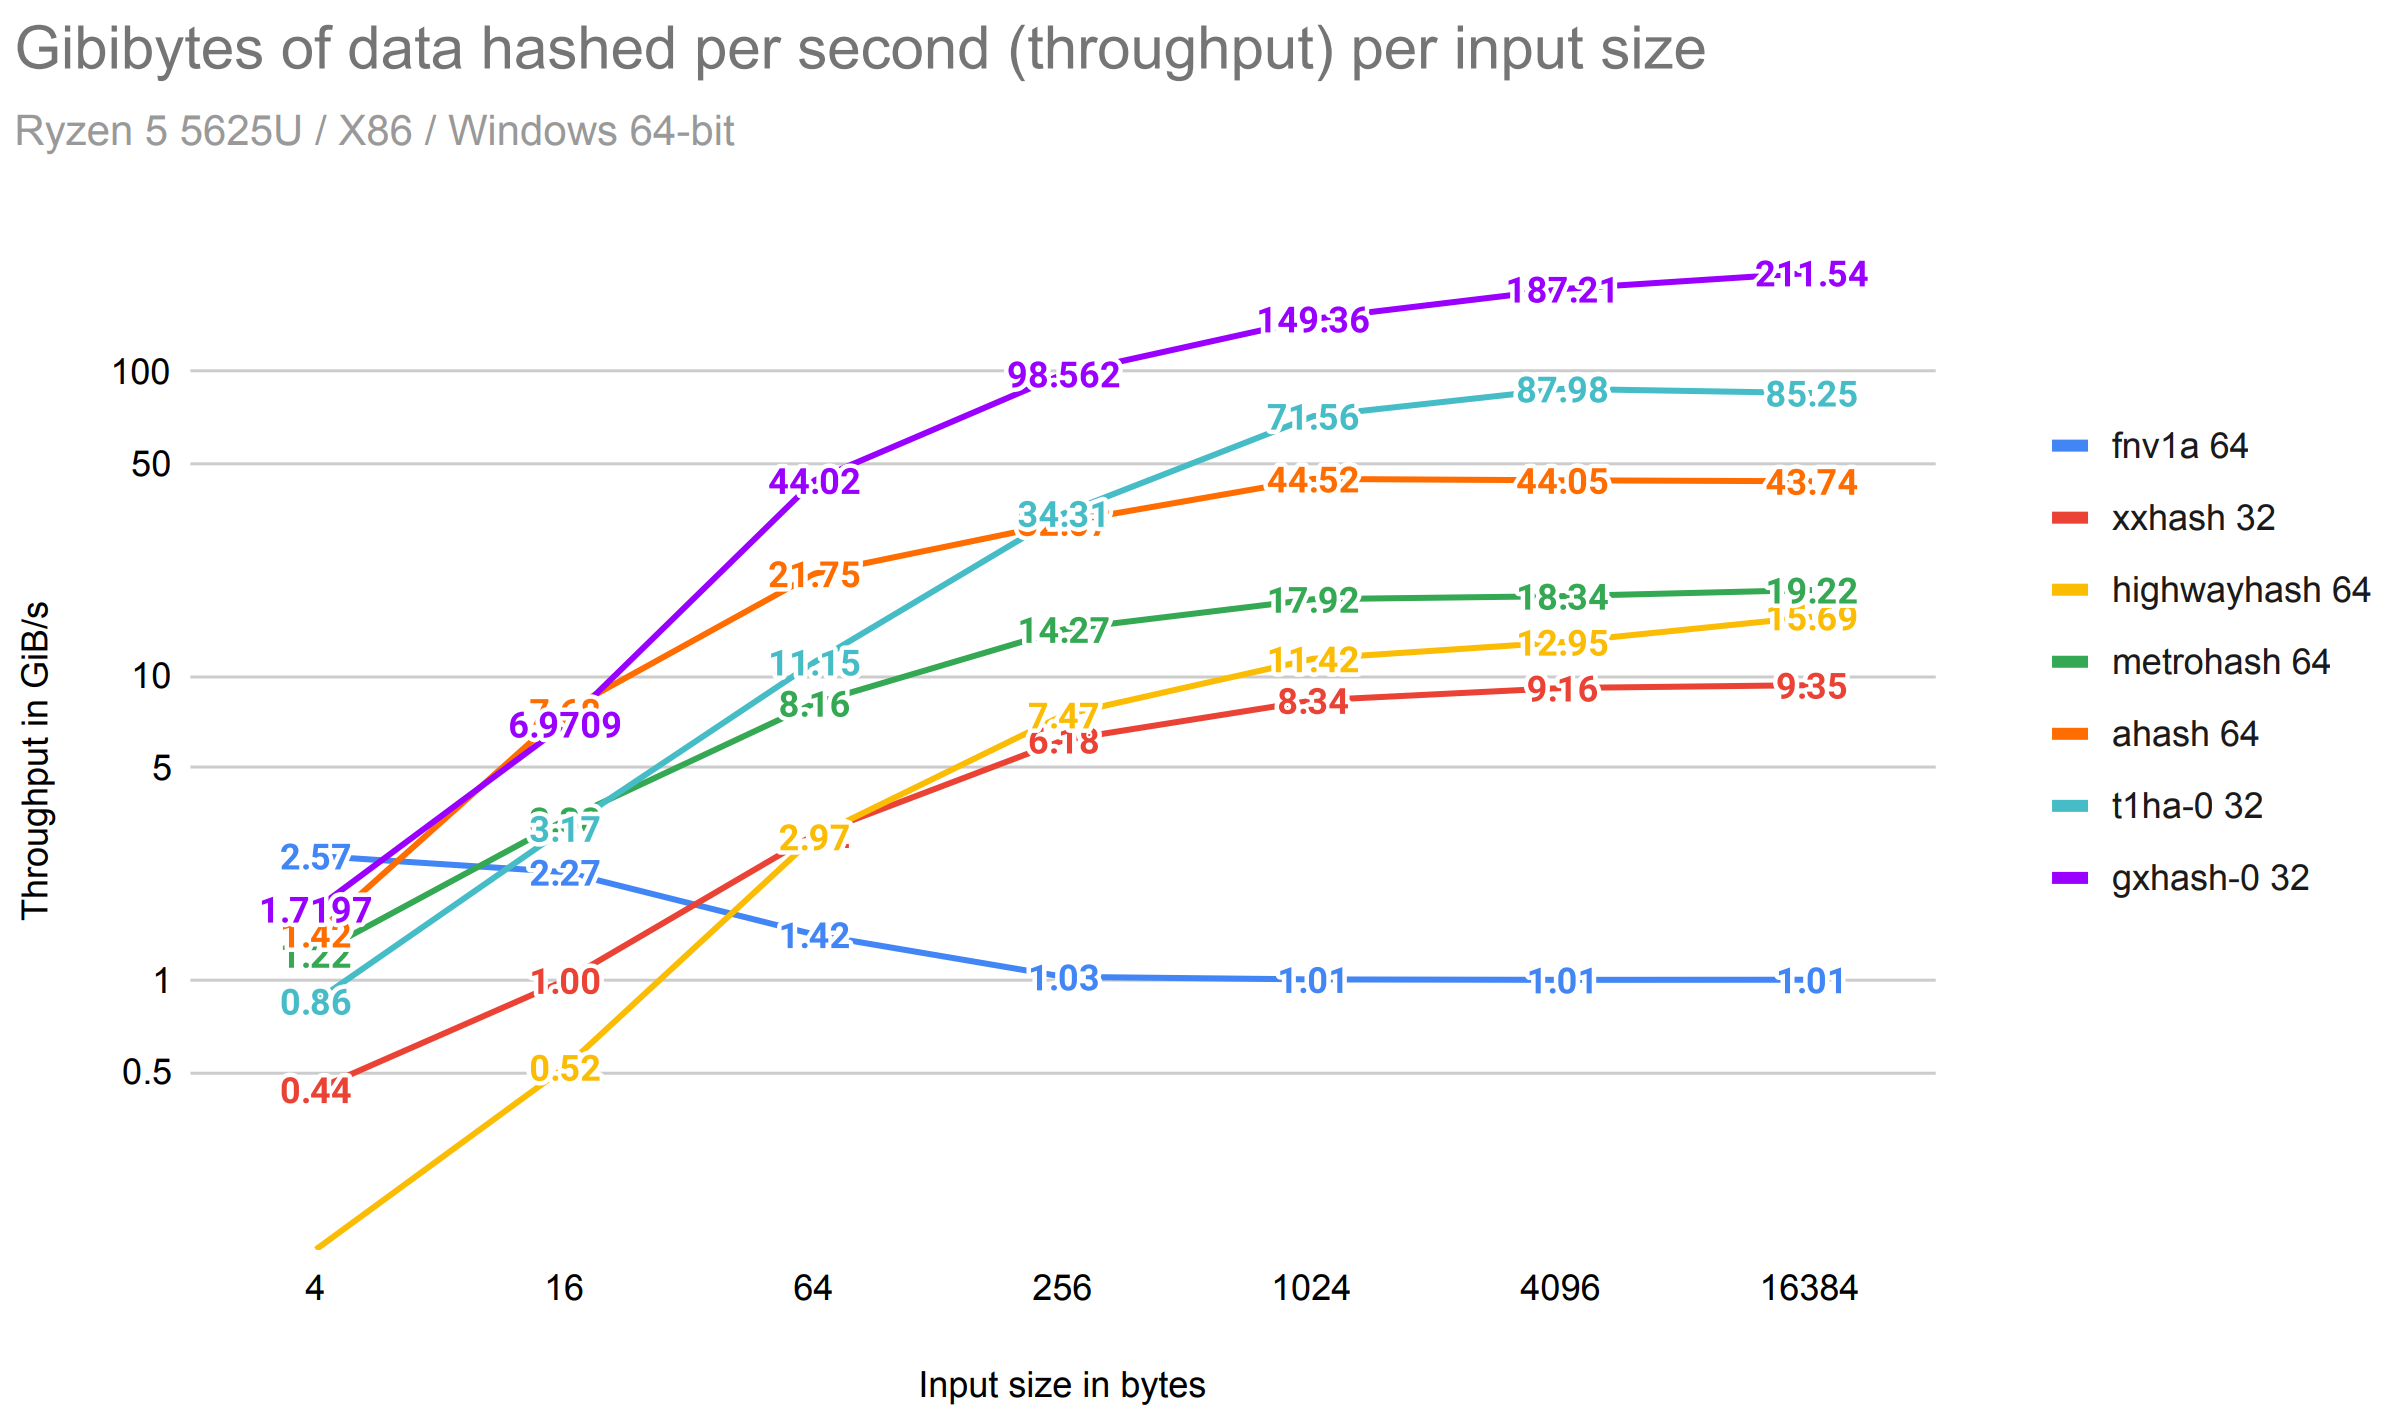
\includegraphics[width=1\textwidth]{throughput.png}
\caption{Mibibytes of data hashed per second (throughput) per input size.}
\label{fig:benchmark-throughput}
\end{figure}

The results are compelling: GxHash consistently outperforms its counterparts, achieving throughput rates that are an order of magnitude higher in many instances. For almost any input size and on all platforms used for the benchmark, the 128-bit state GxHash was the fastest.
The 256-bit GxHash reaches almost two times the maximum throughput of the 128-bit GxHash implementation, as excepted. We can notice however that it performs slightly worse for inputs of small sizes, which can be explained by the overhead of extracting and xoring the two 128-bit parts of the state. Ahash slightly outperforms the 256-bit GxHash for inputs smaller than 128 bytes, but becomes much slower as input size grows.

\paragraph{A word on inlining}\leavevmode\\
On the GCP and Apple M1 Pro benchmarks, the algorithm reaches an impressive 11 Gb/s for 8 bytes inputs. While some algorithms that are supposed to be heavily optimized for small input sizes such as XxHash, they only reach up to a quarter of that throughput. After some analysis, a theory was that assembly code for XxHash was much larger than GxHash, thus preventing the algorithm to be inlined in the benchmark itself. After analysis using cargo asm, it turned out that on ARM XxHash produces 10 times as much assembly than GxHash. Forcing all methods not to be inlined in the benchmarks tend to prove this theory, as timing for small inputs are now all in the same ballpark. Inlining being a important part of the optimization done by compilers is also why special care was taken to make GxHash implementation leading to as little as bytecode as possible. Since criterion.rs benchmarking fixture is also leading the GxHash to be inlined, we think those benchmark results are viable and representative of the real world usage.

\section{Discussion}
\subsection{Limitations}

\subsubsection{Portability}
As previously stated, portability between different state sizes was not a design goal for GxHash. The algorithm functions across a variety of platforms, such as x86 and ARM, with consistent results within the same state size implementation. However, it is important to note that the 128-bit and 256-bit state versions of GxHash will produce distinct hashes for the same input. This discrepancy means that hashes generated by one state size are not directly comparable to those generated by another. To prevent any potential confusion, it is recommended that users choose one state size and maintain consistency throughout the hashing process, especially when hashes may need to be compared or persisted. This limitation is deemed acceptable for use-cases such as in-process hash tables where the state size does not change. Developing a version of GxHash that harmonizes the outputs of different state sizes would involve trade-offs, likely affecting the algorithm’s performance or complexity.

\subsubsection{Compiler Dependencies} 
The Temporal Construction presented in this paper is implemented for GxHash by declaring each lane with its own variable. While it worked at the time of writing (rustc 1.68.0), it is in the end the compiler's responsibility to decide how many registers to use. We cannot exclude that in another context (different version, different language/compiler, ...) the compiler will undo the ILP we tried to implicitly introduce. This could be countered by writing the algorithm directly in assembly code, at the cost of complexity.

\subsection{Future Work}
Despite the outstanding benchmark results, we think there are still many possible paths for research and improvement. Here is a non-exhaustive list:
\begin{itemize}
    \item Leverage larger SIMD intrinsics, such as Intel AVX-512 or ARM SVE2.
    \item Run more quality benchmarks
    \item Analyze security properties.
    \item Rewrite the algorithm in assembly code or a language that is more explicit about registers.
    \item Introduce more than one stage of laning. For instance 16 lanes, then 8 lanes, then 4 lanes, and finally 2 lanes, to leverage ILP as much as possible.
    \item Organize processing loop to result in even less bytecode to be generated, favoring inlining opportunities.
    \item Fine-tune the finalization stage to find the perfect balance between performance and avalanche effect.
\end{itemize}

\section{Conclusion}

By leveraging the capabilities of modern CPUs, such as Single Instruction, Multiple Data (SIMD), GxHash achieves unparalleled throughput, setting a new standard for efficiency and performance amongst non-cryptographic hashing algorithms. A pivotal innovation in this endeavor is the "Temporal Construction," which is specifically designed to harness Instruction-Level Parallelism (ILP), further optimizing the hashing process.

However, it's essential to note that while GxHash offers significant improvements, the behavior of any hash algorithm can be influenced by various factors. As such, potential users should approach with an understanding that results might vary based on specific use cases and input data.\\

The capabilities of GxHash represent a significant step forward in non-cryptographic hashing. In a world where real-time processing is becoming a standard, this algorithm not only enables systems to respond more swiftly but also promotes greater energy efficiency.

\bibliography{references}
\bibliographystyle{plain}

\end{document}
